%%%%%%%%%%%%%%%%%%%%%%%%%%%%%%%%%%%%%%%%%
% BAKALÁŘSKÁ PRÁCE			%
% JAKUB FLAŠKA				%
% Šablona převzata ze stránek KSE	%
% (C) FJFI ČVUT v Praze			%
%%%%%%%%%%%%%%%%%%%%%%%%%%%%%%%%%%%%%%%%%

% Typ dokumentu
\documentclass[a4paper,12pt]{report}	% report - jednostranný tisk

%%%%%%%%%%%%%%%%%%%%%%%%%%%%%%%%%%%%%%%%%%%%%%%%%%%
%% Pouzite balíčky

% Kódování a zpracování ČJ
%\usepackage[czech]{babel}	% cestina
\usepackage[T1]{fontenc}	% balicek fontu
\usepackage[utf8]{inputenc}	% cestina
% Vytvoření indexu a seznamu použité literatury
\usepackage{index}		% vytvoření obsahu
\usepackage[pdftex]{hyperref}	% vygeneruje rejstřík při použití pdflatex
\usepackage{cite}		% vytvoření literatury
\usepackage{multibib}		% více zdrojů literatury
% Práce s obrázky
\usepackage{graphicx}		% obrázky
\usepackage{subfig}		% více obrázků v políčku
% Ostatní
\usepackage{listings}		% vkladani zdrojoveho kodu
\usepackage[usenames]{color}	% použití barevného textu
\usepackage{url}		% zpracování www adresy
\usepackage{verbatim}		% moznost viceradkovych kommentaru prikazem \begin{comment}
\usepackage{array}		%
\usepackage{caption}		% Popisky obrázků jiným písmem, než zbytek textu.
\usepackage{amsmath}
\usepackage[all]{hypcap}
\usepackage{caption}


%%%%%%%%%%%%%%%%%%%%%%%%%%%%%%%%%%%%%%%%%%%%%%%%%%%
%% Formát textu

\oddsidemargin=10mm		% levý okraj
\topmargin=-15mm		% horní okraj
\textwidth=150mm
\textheight=240mm
\pagenumbering{arabic}
\pagestyle{plain}

%\parindent=0pt			% odsazení prvního řádku
\parskip=7pt			% mezera mezi odstavci
\frenchspacing			% typografická pravidla

\renewcommand{\rmdefault}{phv}	% Arial
\renewcommand{\sfdefault}{phv}	% Arial


%%%%%%%%%%%%%%%%%%%%%%%%%%%%%%%%%%%%%%%%%%%%%%%%%%%
% Nastavení balíčků
%%%%%%%%%%%%%%%%%%%%%%%%%%%%%%%%%%%%%%%%%%%%%%%%%%%


%%%%%%%%%%%%%%%%%%%%%%%%%%%%%%%%%%%%%%%%%%%%%%%%%%%%
%% Formátováni zdrojů - cite, Multibib
%Bibtex
\bibliographystyle{plain}		% styl primarnich zdroju

\newcites{sec}{Secondary sources}	% sekundarni zdroje
\bibliographystylesec{plain}		% styl sekundarnich zdroju

%%%%%%%%%%%%%%%%%%%%%%%%%%%%%%%%%%%%%%%%%%%%%%%%%%%
% Vytvoření indexu pro rejstřík a citace - index
%index
\newindex{default}{idx}{ind}{}

%%%%%%%%%%%%%%%%%%%%%%%%%%%%%%%%%%%%%%%%%%%%%%%%%%%
%%%%%%%%%%%%%%%%%%%%%%%%%%%%%%%%%%%%%%%%%%%%%%%%%%%

\DeclareFontShape{OT1}{cmtt}{bx}{n}{cmttb10}{}	% Definování fontu pro bold type-writer.

% Caption
\captionsetup{%font=small,		% Formát popisků.
	format=plain,
	labelfont=bf,
	%textfont=it
}



% Nastavení odkazů - hyperref
\hypersetup{ 
linkbordercolor={1 1 1},	% rámeček kolem odkazu bude bílý
citebordercolor={1 1 1}		% rámeček kolem odkazu citace bude bílý 
} 

% Nastavení balíčku pro vkládání zdrojového kódu - lstlistings
\definecolor{LightGray}{RGB}{245,245,245}
%\definecolor{LightRed}{RGB}{255,100,100}
%\definecolor{LightGreen}{RGB}{70,150,60}
%\definecolor{LightBlue}{RGB}{80,100,240}

\definecolor{LightRed}{RGB}{255,100,100}
\definecolor{LightGreen}{RGB}{60,143,49}
\definecolor{LightBlue}{RGB}{39,62,237}
\definecolor{Purple}{RGB}{162,4,207}


\lstset{ %
language=C++,                % choose the language of the code
basicstyle=\small\tt\color{black},          % print whole listing small
keywordstyle=\small\color{LightBlue},	% bold black keywords
identifierstyle=\small\color{black},           % nothing happens
commentstyle=\small\color{black}, % white comments
stringstyle=\ttfamily,      % typewriter type for strings
showstringspaces=false,     % no special string spaces
numbers=left,                   % where to put the line-numbers
numberstyle=\tiny\tt,      % the size of the fonts that are used for the line-numbers
%stepnumber=2,                   % the step between two line-numbers. If it's 1 each line will be numbered
numbersep=5pt,                  % how far the line-numbers are from the code
%backgroundcolor=\color{LightGray},  % choose the background color. You must add \usepackage{color}
showspaces=false,               % show spaces adding particular underscores
showstringspaces=false,         % underline spaces within strings
showtabs=false,                 % show tabs within strings adding particular underscores
frame=single,			% adds a frame around the code
tabsize=3,	                % sets default tabsize to 2 spaces
%captionpos=b,                   % sets the caption-position to bottom
breaklines=true,                % sets automatic line breaking
breakatwhitespace=false,        % sets if automatic breaks should only happen at whitespace
%title={Zdrojovy kod},                 % show the filename of files included with \lstinputlisting; also try caption instead of title
%escapeinside={\%*}{*)}          % if you want to add a comment within your code
escapechar=!,
}

%\renewcommand{\lstlistingname}{Kód}


\renewcommand{\textfraction}{0.05}
\renewcommand{\topfraction}{0.2}	% max fraction of floats at top
\renewcommand{\bottomfraction}{0.2}	% max fraction of floats at bottom

%\setlength{\topsep}{10pt}
%\setlength{\itemsep}{10pt}

\newcommand{\redlist}[1]{{\color{LightRed}#1}}
\newcommand{\greenlist}[1]{{\color{LightGreen}#1}}

%%%%%%%%%%%%%%%%%%%%%%%%%%%%%%%%%%%%%%%%%%%%%%%%

% Formátování C++ příkazů uprostřed textu
\newcommand{\clist}[1]{\texttt{\hyphenchar\font45\relax #1}} % font s fixní vzdáleností

% Makro pro české uvozovky, použití \uv{...}
\def\bq{\mbox{\kern.1ex\protect\raisebox{-1.3ex}[0pt][0pt]{''}\kern-.1ex}}
\def\eq{\mbox{\kern-.1ex``\kern.1ex}}
\def\ifundefined#1{\expandafter\ifx\csname#1\endcsname\relax }%
\ifundefined{uv}%
        \gdef\uv#1{\bq #1\eq}
\fi

\hyphenation{Open-GL}

%%%%%%%%%%%%%%%%%%%%%%%%%%%%%%%%%%%%%%%%%%%%%%%%%%%%%%
%%%%%%%%%%%%%%%%%%%%%% BAKALARSKA PRACE %%%%%%%%%%%%%%
%%%%%%%%%%%%%%%%%%%%%%%%%%%%%%%%%%%%%%%%%%%%%%%%%%%%%%

%%%%%%%%%%%%%%%%%%%%%%%%%%%%%%%%%%%%%%%%%%%%%%%%%%%%
%%%%%%%%%%%%%%%%%%%%%% POJMY  %%%%%%%%%%%%%%%%%%%%%%            

\newcommand{\cvut}{Czech Technical University in Prague}
\newcommand{\fjfi}{Faculty of Nuclear Sciences and Physical Engineering}
\newcommand{\km}{Department of Mathematics}
\newcommand{\obor}{Inženýrská informatika}
\newcommand{\zamereni}{Tvorba software}
\newcommand{\nazevcz}{Softwarový nástroj pro manipulaci s daty z magnetické rezonance a jejich vizalizaci}
\newcommand{\nazeven}{Development of a Software Instrument for MRI Data Manipulation and Visualization }     
\newcommand{\autor}{Bc.~Jakub Flaška}
\newcommand{\rok}{2011}
\newcommand{\vedouci}{Ing.~Pavel Strachota} 

%%%%%%%%%%%%%%%%%%%%%%%%%%%%%%%%%%%%%%%%%%%%%%%%

%%%%%%%%%%%%%%%%%%%%%% UVODNI STRANA  %%%%%%%%%%%%%%%%%%%%%%

\begin{document}
\begin{comment}

\thispagestyle{empty}

\begin{center}
	{\fontsize{15}{15.5} \bf \cvut\\[2mm] \fjfi \\[2mm] \km}	% Název školy, fakulta
	\vfill
		\begin{center}
			
\includegraphics[width=50mm]{Text/IMG/00_Logo_CVUT_bw.jpg}	% Logo
		\end{center}
	\vfill
		{\fontsize{35}{36.5} \bf MASTER'S THESIS}		% BAKALÁŘSKÁ PRÁCE
	\vfill			
		{\fontsize{20}{20.5} \bf \nazeven}	% Název práce
	\vfill	
		{\large %\em %\bf								
			\begin{tabular}{rl}
				Author 		& {\bf	\autor}			\\					% Autor
				Supervisor 	& {\bf	\vedouci }		\\					% Školitel
				Academic year		& {\bf	\rok }			\\					% Rok
			\end{tabular}
		}
\end{center}


\begin{comment}
%%%%%%%%%%%%%%%%%%%%%% PROSTOR PRO ZADANI  %%%%%%%%%%%%%%%%%%%%%%
\newpage
\thispagestyle{empty} Sem vložit list s podepsaným zadáním od děkana, jakožto jediný oboustranný list.


%%%%%%%%%%%%%%%%%%%%%% PROHLASENI %%%%%%%%%%%%%%%%%%%%%%
\newpage
\thispagestyle{empty}

~
\vfill % prázdné místo

{\bf Prohlášení}

\vspace{0.5cm} % vertikální mezera
Prohlašuji, že jsem svou bakalářskou práci vypracoval samostatně a použil jsem pouze literaturu uvedenou v přiloženém seznamu.

Nemám závažný důvod proti užití tohoto školního díla ve smyslu \S60 Zákona č.121/2000 Sb. o právu autorském, o právech souvisejících s právem autorským a o změně některých zákonů (autorský zákon).


\vspace{5mm}V Praze dne ....................\hfill
	\begin{tabular}{c}
	........................................\\ 
	\autor
	\end{tabular}


%%%%%%%%%%%%%%%%%%%%%% PODEKOVANI %%%%%%%%%%%%%%%%%%%%%%
\end{comment}
\begin{comment}%%%%%%%%%%%%
\newpage
\thispagestyle{empty}

~
\vfill % prázdné místo

{\bf Acknowledgment}

\vspace{5mm} % vertikální mezera
I would really like to thank my supervisor Ing. Pavel Strachota for his outstanding help while creating this diploma thesis and my previous work.

\begin{flushright}
\autor
\end{flushright}


%%%%%%%%%%%%%%%%%%%%%% ABSTRAKT %%%%%%%%%%%%%%%%%
\end{comment}%%%%%%%%%%%
\begin{comment}
\newpage
\thispagestyle{empty}

% příprava:\usepackage{subfig}
\newbox\odstavecbox
\newlength\vyskaodstavce
\newcommand\odstavec[2]{
    \setbox\odstavecbox=\hbox{
         \parbox[t]{#1}{#2\vrule width 0pt depth 4pt}}
    \global\vyskaodstavce=\dp\odstavecbox
    \box\odstavecbox}
\newcommand{\delka}{120mm}


\newcommand{\pracovisteVed}{\km,\\ \fjfi,\\ \cvut}

\newcommand{\konzultant}{}
\newcommand{\pracovisteKonz}{}

\newcommand{\klicova}{programování, GUI, grafické uživatelské rozhraní, C++, Qt, DICOM}
\newcommand{\keywords}{programming, GUI, graphic user interface, C++, Qt, DICOM}   



{\noindent \bf \large Abstract} \\[5mm]
\begin{tabular}{l p{10cm}}
	{\em Master's Thesis}	& 	\\[1mm]
	{\em Title:}	& \nazeven	\\[1mm]
	{\em Author:}	& \autor	\\[1mm]
	{\em Program:} 	& \obor		\\[1mm]
	{\em Supervisor:}& \vedouci	\\
				& \km		\\
				& \fjfi		\\
				& \cvut		\\[1mm]
	{\em Keywords:}	& \odstavec{\delka}{\keywords}	\\
\end{tabular}

This Diploma Thesis describes development of a C++ application, which is used for displaying images caputured on Magnetic Resonance Imaging unit. Prior to this work, the application was partly implemented. This work sets a few goals: redesign the rendering part of the application, implement Multi-planar recontruction and a system for additional plugins. In addition, the thesis focuses on GUI applications programming and compilation of C++ applications in Win32.


\vspace{10mm}
{\noindent \bf \large Abstrakt} \\[5mm]
\begin{tabular}{l p{10cm}}
	{\em Diplomová práce}	& 	\\[1mm]
	{\em Název:}	& \nazevcz	\\[1mm]
	{\em Autor:}	& \autor	\\[1mm]
	{\em Keywords:}	& \odstavec{\delka}{\klicova}	\\
\end{tabular}

Tato diplomová práce se zabývá vývojem programu sloužícího pro zobrazování snímků z magnetické resonance. Na začátku této práce již byla aplikace částečně implementována. Tato diplomová práce se snaží zejména o následující úkoly: kompletně přepsat část aplikace věnující se vykreslování; implementovan systém zobrazení označovaný jako multiplanární rekonstrukce; přidat do aplikace rozhraní umožňující používání přídavných modulů k aplikaci. Dále se pak práce věnuje v obecnější rovině programování aplikací s grafickým uživatelským rozhraním a shrnuje poznatky o překladu C++ aplikací v prostředí Win32.






\end{comment}
\begin{comment}%%%%%%%%%%%%
%%%%%%%%%%%%%%%%%%%%%% OBSAH %%%%%%%%%%%%%%%%%%%%%%
\newpage
\tableofcontents


%%%%%%%%%%%%%%%%%%%%%%  TEXT PRÁCE %%%%%%%%%%%%%%%%%%%%%%%%%%%%%%%%%%%%%%%%%%%%

\chapter{Introduction}
\vspace{-10mm}
The aim of this Diploma Thesis is development of a C++ application used for viewing Magnetic Resonance data. The task was given by IKEM institute\footnote{Institute for Clinical and Experimental Medicine \cite{ikem}} and was started in work \cite{neskudla} and followed in works \cite{flaska_bc} and \cite{flaska_vu}. The application (further called ``Dicom-Presenter'') allows to open MRI images and offers unique displaying features required by IKEM.

This Diploma Thesis sets three goals to be done: handle project compilation, rewrite application rendering engine and implement new features. The project compilation process needed to be reviewed and automated. There were dependencies on five external libraries which complicated project deployment. Therefore, the rendering part of the application had to be rewritten to remove project dependency on 3rd party libraries like OpenGL\citesec{openglhome}, Cg toolkit\citesec{cgtoolkit}, plib\citesec{plibhome}. Lastly, multi-planar reconstruction\footnote{A multi-planar reconstruction is a way for displaying three-dimensional images. Three slices in three perpendicular planes are displayed. See Chapter \ref{multiplanar}.} and image segmentation were added into the application.


\end{comment}
\chapter*{Dicom-Presenter}
\addcontentsline{toc}{chapter}{Dicom-Presenter}
\vspace{-10mm}

My predecessor Bc. Pavel Neskudla started development of an application for viewing images from MRI as a part of his master's thesis\cite{neskudla}. It was a task given by IKEM institute in Prague\footnote{Institute for Clinical and Experimental Medicine}. IKEM institute specialists found out that they would utilize some application which would allow them to open MRI images elsewhere than only on Siemens computers located in their institute. They would prefer some application where they could view recorded images on their own personal computers. It is possible to find such applications distributed by local developers, but only a few of them reach satisfactory quality requirements. These are definitely commercial applications, so user has to pay. There is also a lot of non-commercial, freeware applications, but functionality of these applications is often limited\cite[page~9]{flaska_bc}. For example, it was not possible to find an application which could open several images at the same time and view them on one screen. Therefore, specialists from IKEM institute decided to ask our faculty to develop such an application which would fit their needs.

\begin{figure}
	\begin{center}
	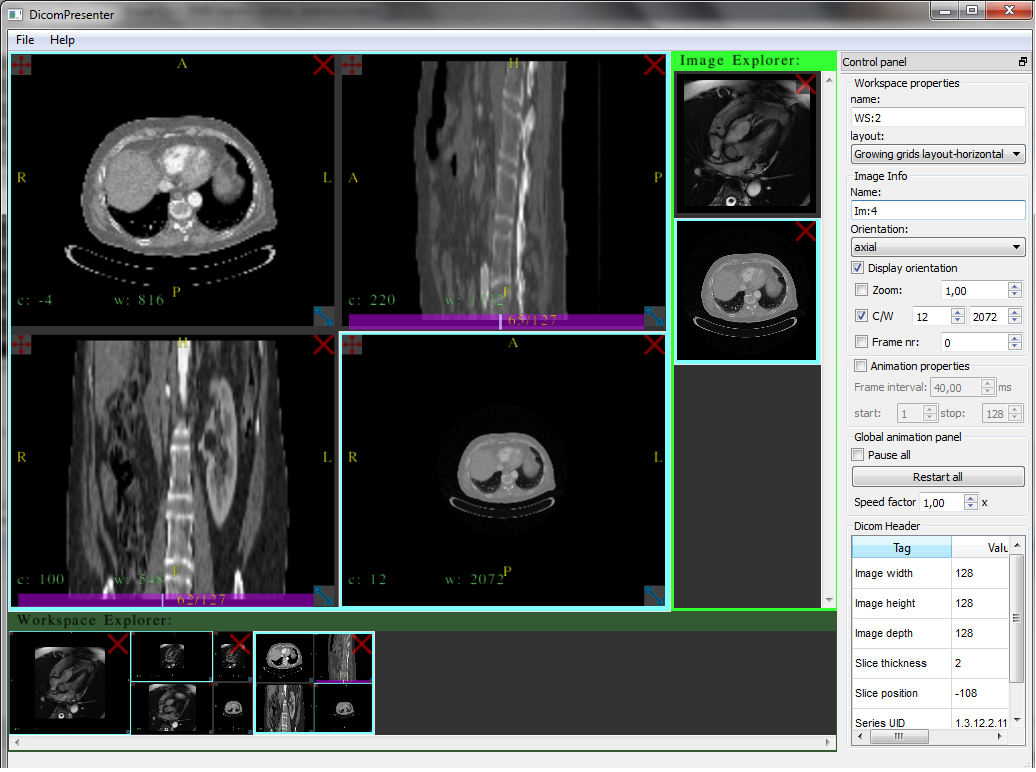
\includegraphics[width=130mm]{Text/IMG/04_GUI_Screenshot.png}
	\end{center}
	\caption{Screenshot of Dicom-Presenter user interface.}
	\label{screenshot}
\end{figure}

\section*{Application requirements}
\addcontentsline{toc}{section}{Application requirements}
The IKEM specialists asked for a typical DICOM images viewer with few more specific features which they missed in freeware programs. A typical DICOM viewer allows you to open .dcm files and display it. .dcm file in this case is a jpeg image equipped with special header including patient's information. There you can see a 2D picture of some part of the patient's body. Some DICOM viewers allow you to open series of .dcm files, which can actually fit into a three-dimensional picture. Less commonly it can be a time animation of organ behaviour in short time period (f.e. one heart beat). DICOM viewers often have some more functions but it is very individual.

There have been two more specific requirements on application functionality by IKEM specialists. They missed certain functions in freeware DICOM applications. The most important function was a possibility to open several images at one time and display them on one screen. The user should be allowed to arrange images on screen to any possible layout he prefers. This functionality allows physicians to see two or more different MRI images on screen so they can easily determine pathological differences among observed organs. It is useful for studying, or teaching.

There have been also requirements that the application should be able to record user's manipulation with images as a video. Then physician can prepare his presentation of images at home and then play the video in front of crowds.

\begin{table}[ht]
	\caption{DICOM viewers.}
	\centering
	\begin{tabular}{cc}
			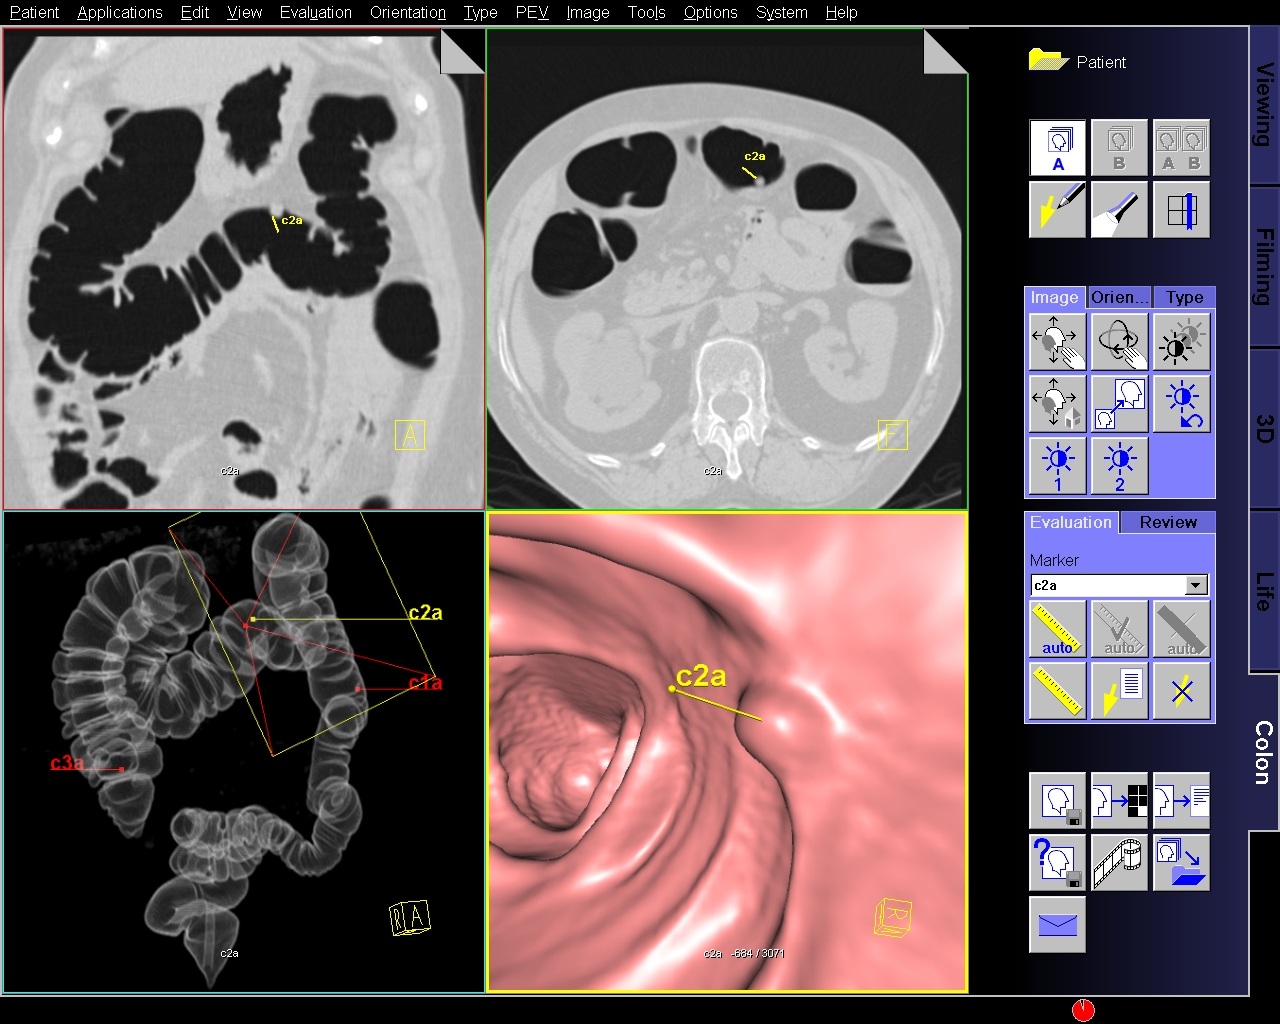
\includegraphics[width=0.5\textwidth,height=0.375\textwidth]{Text/IMG/01_Siemens.jpg}
		&
			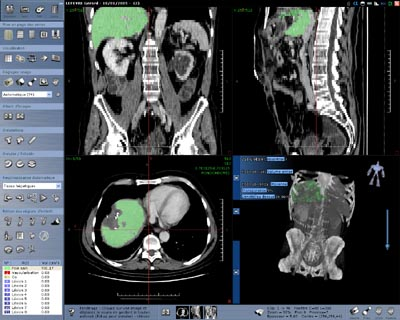
\includegraphics[width=0.5\textwidth,height=0.375\textwidth]{Text/IMG/01_Myrian.jpg}
		\\
			syngo Imaging~\citesec{siemens} & Myrian~\citesec{intrasense}	
		\\
			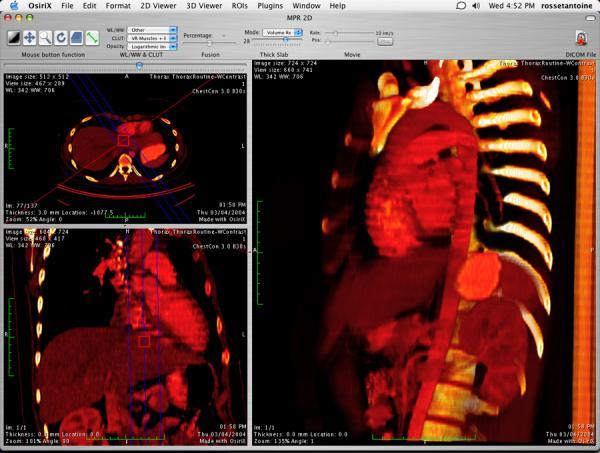
\includegraphics[width=0.5\textwidth,height=0.375\textwidth]{Text/IMG/01_OsiriX.jpg}
		&
			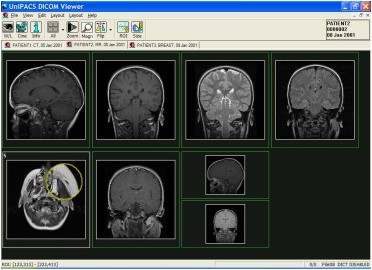
\includegraphics[width=0.5\textwidth,height=0.375\textwidth]{Text/IMG/01_UniPACS.jpg}
		\\
			OsiriX~\citesec{osirix} & UniPACS~\citesec{unipacs}
		\\
		\end{tabular}
\end{table}%

\section*{Application functionality}
\addcontentsline{toc}{section}{Application functionality}
\chapter{Graphic User Interface Programming}
\vspace{-10mm}

A Graphic User Interface (GUI) of an application has to be described in its source code - control elements' layout and their interaction. Each operation system offers its own library for GUI programming. To ease the programming process, additional libraries can be used - libraries, which are focused mainly on creating application's GUI are called Widget Toolkits.

The native libraries for GUI programming are for example Windows API in Windows and xlib in Linux/Unix systems. The process of programming application's GUI with use of only native OS library is following text explained on Windows API. Object-oriented GUI programming is explained with use of Qt\citesec{qthome} and GTK\citesec{qthome} libraries.

\section{GUI programming in Windows API library}
\label{noqt}
Creating an application's GUI with use of only OS related library is quite complicated. The native libraries are simple - both Windows API and xlib are not object-oriented. The application behavior has to be solved by procedural declarations in the source code.

The GUI programming in WinAPI uses following basic elements\cite[Chapter~2]{eventloopprogramming}:

\begin{itemize}
\item Object
\item Object's Procedure
\item Message
\item Message Queue
\item Message Loop
\end{itemize}

The basic idea is following:

\begin{itemize}
\item The core of the application is the Message Loop. It loads messages from the Message Queue and redirects them to proper Objects.
\item Each Object owns a Procedure. The Procedure receives a message and adds the response to Message Queue.
\end{itemize}

This concept is called event-driven programming. There is an example of event-driven application on Listing \ref{WinAPI}. The application loop is located on line \ref{lst:ProgramLoop}. The \clist{GetMessage} functions reads a message from the Message Queue. The \clist{DispatchMessage} forwards the message to propriate object.

The only visible object of the example application is a window created on line \ref{lst:window}. The procedure of the window, which solves its received messages is defined on line \ref{lst:WndProc}.

The \clist{main} function of the application is replaced by the \clist{WinMain} function. So the application course is following: the window is created and the loop starts running; if the user clicks on the window, a message is added to the queue; the message is readed from the queue and then forwarded to the application itself or back to the window.\cite[Chapter~2]{eventloopprogramming}

\begin{lstlisting}[label=WinAPI,caption={An example of a simple application using Windows API for GUI rendering.\protect\cite{WinAPIexample}},escapeinside={@}{@}]
@\label{lst:WndProc}@LRESULT CALLBACK WndProc(HWND hwnd, UINT msg, WPARAM wParam, LPARAM lParam){
    switch(msg){
        case WM_CLOSE:
            DestroyWindow(hwnd);
        break;
        case WM_DESTROY:
            PostQuitMessage(0);
        break;
        default:
            return DefWindowProc(hwnd, msg, wParam, lParam);
    }
    return 0;
}
@\label{lst:WinMain}@int WINAPI WinMain(HINSTANCE hInstance, HINSTANCE hPrevInstance,
    LPSTR lpCmdLine, int nCmdShow){
    WNDCLASSEX wc;
    HWND hwnd;
    MSG Msg;
    //Step 1: Registering the Window Class
    wc.cbSize        = sizeof(WNDCLASSEX);
    wc.style         = 0;
    wc.lpfnWndProc   = WndProc;
    wc.cbClsExtra    = 0;
    wc.cbWndExtra    = 0;
    wc.hInstance     = hInstance;
    wc.hIcon         = LoadIcon(NULL, IDI_APPLICATION);
    wc.hCursor       = LoadCursor(NULL, IDC_ARROW);
    wc.hbrBackground = (HBRUSH)(COLOR_WINDOW+1);
    wc.lpszMenuName  = NULL;
    wc.lpszClassName = g_szClassName;
    wc.hIconSm       = LoadIcon(NULL, IDI_APPLICATION);
    // Step 2: Creating the Window
 @\label{lst:window}@   hwnd = CreateWindowEx(
        WS_EX_CLIENTEDGE,
        g_szClassName,
        "The title of my window",
        WS_OVERLAPPEDWINDOW,
        CW_USEDEFAULT, CW_USEDEFAULT, 240, 120,
        NULL, NULL, hInstance, NULL);
    // Step 3: The Message Loop
@\label{lst:ProgramLoop}@    while(GetMessage(&Msg, NULL, 0, 0) > 0){
        TranslateMessage(&Msg);
        DispatchMessage(&Msg);
    }
    return Msg.wParam;
}
\end{lstlisting}

Programming GUI applications in plain WinAPI requires necessary steps to be done, such as: defining the main loop, assigning a procedure to the object, etc. All these steps are ensured by Widget Toolkits, if used. 

\begin{comment}

\section{GUI programming in Windows API}
Development of GUI application for Windows is possible with Windows API. This is the name given to a set of various APIs - communication interfaces for performing services. These communication interfaces offer manipulation with file-system, devices and also creating graphic windows.

Most common parts of Windows API are:
\begin{itemize}
\item \clist{kernel32.dll}, which is needed for memory management, input/output, process and thread creation.
\item \clist{user32.dll} for creating GUI elements, such as windows, buttons, etc.
\item \clist{shell32.dll} which offers access to Windows command line
\item \clist{WinSock} to use network
\end{itemize}
\end{comment}

\section{Widgets Toolkits}
\label{guiframeworks}
Widgets Toolkits are libraries designed to ease GUI application creation. Complicated widget declaration processes are encapsulated inside the library. Then, library classes are used instead of calling OS related functions. Examples of currently popular Widgets Toolkits can be Qt\citesec{qthome} and GTK\citesec{gtkhome} libraries\cite[pages~413-416]{qtvsgtk}.

Both Qt and GTK are based on the same schema. All control elements are represented by library classes. The control elements can be easily added to application windows. Control functions describing application response to user actions are defined. Then the control elements and control functions are connected together.

Source code syntax of Qt library and GTK library is very similar. Examples of two identical applications using GTK and Qt can be found on Listings \ref{gtk} and \ref{qt}. Both applications create a simple window with a button inside. Clicking the button writes a console output. The button and window creation can be found on lines \ref{lst:gtkbuttonstart} - \ref{lst:gtkbuttonfinish} on Listing \ref{gtk} (GTK) and lines \ref{lst:qtbuttonstart} - \ref{lst:qtbuttonfinish} on Listing \ref{qt} (Qt). The process is very similar unlike Qt uses functions in its classes and GTK uses global functions. The command on lines \ref{lst:gtkconnect} (Listing \ref{gtk}) and \ref{lst:qtconnect} (Listing \ref{qt}) is used for setting up interaction between button click and proper function call. The main difference is that GTK allows connection to global function calls (line \ref{lst:gtkcall}, Listing \ref{gtk}), unlike Qt allows calling functions of object inheriting QObject class (line \ref{lst:gtkcall}, Listing \ref{qt}).

\begin{lstlisting}[label=gtk,caption={A sample application using GTK library.\protect\cite{gtktutorial}},escapeinside={@}{@}]
@\label{lst:gtkcall}@static void message(GtkWidget *widget, gpointer data){
    cout << "Hello World!";
}
...
@\label{lst:gtkbuttonstart}@GtkWidget *window = gtk_window_new (GTK_WINDOW_TOPLEVEL);
GtkWidget *button = gtk_button_new_with_label ("Hello World");
GtkWidget *layout = gtk_fixed_new();
gtk_fixed_put(GTK_FIXED(layout), button);
@\label{lst:gtkbuttonfinish}@gtk_container_add(GTK_CONTAINER(window), layout);
@\label{lst:gtkconnect}@g_signal_connect (button, "clicked", G_CALLBACK (message), NULL);
\end{lstlisting}

\begin{lstlisting}[label=qt,caption={A sample application using Qt library.},escapeinside={@}{@}]
@\label{lst:qtcall}@class callhandler : public QObject {
Q_OBJECT
public slots:
	void message () {
		cout << "Hello World!";
	}
}
...
@\label{lst:qtbuttonstart}@QWidget *window = new QWidget();
QPushButton *button = new QPushButton();
QLayout *layout = new QGridLayout();
layout->add(button);
@\label{lst:qtbuttonfinish}@window->setLayout(layout);
@\label{lst:qtconnect}@connect(button,SIGNAL(clicked()),callhandler,SLOT(message()));
\end{lstlisting}
\chapter{Image manipulation}
\vspace{-10mm}

Dicom-Presenter is an application for viewing image data. Entire image manipulation was solved with use of OpenGL library in early version of Dicom-Presenter. OpenGL was used for image storing, for changing image properties and for drawing images on screen. Unfortunately, OpenGL brought complications to application compatibility with various hardware. Therefore, author of this work decided to remove OpenGL from application and replace all classes using OpenGL with their non-OpenGL equivalents. 

Before rewriting all image processing classes without OpenGL it was a need to study how to complete all image processing tasks without OpenGL. Moreover, OpenGL uses GPU to perform its tasks so it was a need to calculate the loss of performance when OpenGL will be removed. 

\section{Image storing}
\label{rawdata}
There are two different libraries used for image manipulation in Dicom-Presenter. DCMTK library is used for loading images from hard disk, while Qt library (formerly OpenGL) is used for displaying images on computer screen. DCMTK library must be used since it supports loading files in DICOM format, moreover some application framework must be used for image displaying. DCMTK library offers loading compressed image files and saving them uncompressed into RAM memory. To be able to display these raw data properly by Qt library, it is mandatory to understand the way image data are represented in computer. 

A color image consisting of $m \cdot n$ points (pixels) can be described by $m \cdot n$ number triads. The triads would be coordinates in RGB or HSV color space \footnote{Colors which can be displayed can be fully described by three values. This fact is based on human eye anatomy and leads to construction of coordinate systems describing each displayable color. Coordinates of RGB color space are red, blue, green color while hue, saturation, value are coordinates in HSV color space.}. Data in a computer are stored in elementary units - bytes, which can hold 256 different values. Each byte consists of eight unitary units - bits ($2^8 = 256 $). If considered that one byte can include color information of only one pixel, then only eight-bit multiples can be used for a pixel color storage: 8 bits, 16 bits, 24 bits, etc. In case of 24 bit color depth, three bytes are used for a pixel color storage - each byte for each color. If 8 bits depth or 16 bits depth is used, in both cases the bit numbers are not divisible by three, so there are several ways of how to distribute bits among colors.
 
Qt library uses three different formats of 16 bit color information storage. The formats differ by number of bits distributed to each color and are described by triads of numbers: 5-6-5, 5-5-5, 4-4-4. The first format uses 5 bits for red color, 6 bits for green color and 5 bits for blue color. The numbers of bits for each color are uneven but no redundant bits are present. Both 5-5-5 and 4-4-4 formats include redundant bits for each image pixel.

Qt library allows displaying images which are actually saved in computer memory as an array of bytes in some of supported formats (such as described above). Next to color depth formats, image storage can differ by number of bytes used for storing each image line. If an image has $m \cdot n$ pixels and two bytes are used per pixel (f.e. 16 bit 5-5-5), there is no rule that $m \cdot n \cdot 2$ bytes will be used. A computer memory in x86 architecture reads its data in elements called words usually consisting of 4 bytes for x86 architecture and 8 bytes for 64-bit architecture. Therefore, image data are in computer memory often aligned that each image line starts at a beginning of some 4-byte or 8-byte word. For instance, if we consider an image of $100 \cdot 100$ pixels saved with 8 bit pixel depth on 64-bit architecture, each line consisting of $100$ pixels would be saved on $128$ or bytes.

In conclusion, if a picture is reconstructed from uncompressed raw data saved in computer memory, essential indications are which color storage format is used for each pixel and which bit align is used for each pixel-line. Those two information are enough for correct image reconstruction.

\subsection{Image construction from raw data in Qt library}
As said in previous text, DCMTK library allows loading compressed files from hard disk and saves them into RAM memory in one of mentioned data alignment. Qt library allows displaying the image data onto computer screen. It is mandatory to coordinate an output of DCMTK and an input of Qt library to be able to display an image properly.

DCMTK library offers a function which saves a copy of loaded image data into a new place in image memory in required data alignment. The function declaration is:

\clist{const void* DicomImage::getOutputData	(const int bits = 0,
const unsigned long frame = 0,
const int planar = 0 )}

The first parameter denotes a required data alignment of each pixel; the other two parameters describe the orientation of the image slice inside the three-dimensional texture. The function returns a pointer to the part of memory where image data will be stored.

Besides, Qt library offers a construction of its object depending on image data already stored in computer memory. The object receives a pointer to image data through its constructor. If the image data meet prospective requirements, the object can be called to draw the image at any time, as long as the data are still on the place in computer memory.

The constructor declaration is:

\clist{QImage::QImage(uchar* data, int width, int height, int bytesPerLine, Format format)}

The first parameter is a pointer to image data already saved in computer memory. The data are declared as \clist{unsigned char} which is a C++ equivalent of a \clist{byte} type. The last parameter \clist{format} describes a pixel alignment. It describes a number of bytes used for each pixel and a particular way of color information storage. The \clist{bytesPerLine} parameter describes an image line alignment of pixel data.

Qt library itself cannot determine the exact values of above described parameters. Therefore, the parameter values must be known before. A misleading value of parameter describing pixel color storage will lead to false color interpretation of the image. Furthermore, incorrect parameter describing image line alignment can avert image loading or can cause a program failure due to unauthorized memory access.  


\begin{figure}
	\begin{center}
	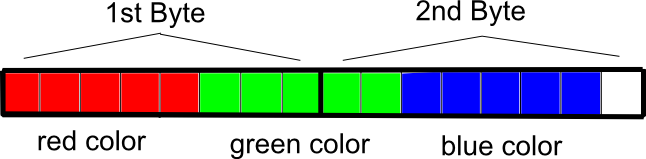
\includegraphics[width=130mm]{Text/IMG/ImageStoring_16bit.png}
	\end{center}
	\caption{A distribution of 16 bits of 2 bytes among three colors of a pixel.}
	\label{imagestoring}
\end{figure}

\section{Image enhancement operations}
\label{brightnesscontrast}

One of important tasks to re-implement in Dicom-Presenter was an ability to adjust image brightness and contrast. Images which will be opened in Dicom-Presenter can be captured on various MRI units with various imaging properties. The ability to increase image brightness and contrast is mandatory to ensure sufficient display quality. Too dark or too gray images need to be brightened or need to increase contrast to ensure better observation of physiological findings. A brightness and contrast change is among DICOM users called ``windowing''.

For further needs of this text brightness and contrast need to be defined. 

A gray-scale image can be considered as a matrix of numbers: 

\[
 Im_{res_{x},res_{y}} =
 \begin{pmatrix}
  Im(1,1) & Im(1,2) & \cdots & Im(1,res_{x}) \\
  Im(2,1) & Im(2,2) & \cdots & Im(2,res_{x}) \\
  \vdots  & \vdots  & \ddots & \vdots  \\
  Im(res_{y},1) & Im(res_{y},2) & \cdots & Im(res_{y},res_{x})
 \end{pmatrix}
\]

where $ res_{x} $, $res_{y}$ are dimensions of the image. $Im(x,y)$ is a lightness of a pixel.

Brightness then can be defined as:
\[
  Brightness(Im) = \frac{1}{res_{x}  \cdot res_{y}}\sum_{\substack{0 \leq x \leq res_{x} \\ 0 \leq y \leq res_{y}}} Im(x,y)
\]

Contrast is understood as overall difference in luminosity between bright and dark pixels. There are more possible definitions of contrast. One possible definition is:

\[
Contrast(Im) = \sqrt{\frac{1}{res_{x} \cdot res_{y}}\sum_{\substack{ 0 \leq x \leq res_{x} \\ 0 \leq y \leq res_{y} }}(Im_{x,y}-Brightness(Im))^2}
\]

An argument for using these two definitions for brightness and contrast is that they are analogies for mean value and variance of set of values.

If there is a need of increasing or decreasing image brightness in computer applications simply a constant is added to all image points:

\begin{equation}
\label{brightness}
  Im(x,y) \longmapsto Im(x,y) + c_{brightness} 
\end{equation}

Image contrast is usually adjusted by a linear transformation applied to all image points:

\begin{equation}
\label{contrast}
  Im(x,y) \longmapsto   (Im(x,y) - 0.5) \cdot c_{contrast} + 0.5
\end{equation}

A disadvantage of both ways is that some image information is lost. Let's consider an image described by a matrix with elements of integers in range from zero to 255. Let the brightness of the picture increased according to formula \eqref{brightness} with a positive constant $ c_{brightness} $. Then all the points brighter than $ 255 - c_{brightness} $ on original image will have luminosity of 255 regardless their original luminosity. Similarly if contrast would be increased according to formula \eqref{contrast} with a constant $ c_{contrast} $ then all points brighter than $ \frac{1}{2} \cdot 255 \cdot (\frac{1}{c_{contrast}}+1) $ will have the same color (maximum white). As well all pixels darker than $ \frac{1}{2} \cdot 255 \cdot (1 - \frac{1}{c_{contrast}}) $ will have the same color (maximum black).

\clist{krivka na nelinearni kontrast z vyzkumaku}

\subsection{Pixel manipulations in Qt}

Qt library doesn't offer its own functions for elementary pixel manipulations such as change of brightness and contrast. These operations (described in Section \ref{brightnesscontrast}) must be done in application source code for each image pixel.

A change of brightness or contrast of an image of $m \cdot n$ pixels will be done in $m \cdot n$ steps. In each step a color of the pixel must be obtained, new color value will be calculated and the value will be saved into the picture. Qt library offers two ways to perform the task: pixel manipulation functions or direct memory access.

If pre-implemented Qt pixel manipulation functions are used, the source code will be following:

\begin{lstlisting}[label=qtcontrast,caption={Image enhancement operations implementation using Qt library functions for pixel manipulation.},escapeinside={@}{@}]
QImage image(...);
for (int y=0; y<height; y++) {
	for (int x=0; x<width; x++) {
		@\label{lst:pixel}@QRgb color = image.pixel(x,y);
		@\label{lst:operation}@QRgb newcolor = qRgb(func1(qRed(color)),func2(qGreen(color)),func3(qBlue(color)));
		@\label{lst:setPixel}@image.setPixel(x,y,color);
	}
}
\end{lstlisting}

Function \clist{QRgb QImage::pixel(int x,int y)} is used to retrieve color information of a pixel. The code on line \ref{lst:operation} performs a color manipulation. Function \clist{void QImage::setPixel(int x,int y,QRgb rgb)} is used to save the color information back to the picture. Due to multi-thread programming support the \clist{QImage::setPixel} function offers low performance. Within each function call Qt library must attach and detach a process to shared memory segment where the image data are stored. These steps are performance expensive.

Nevertheless, Qt library offers a high performance option to change image pixel data. Image data are modified directly inside the computer memory without a function call from QImage class. A function from QImage class is called just to retrieve a pointer to memory segment containing image data. The code will be following:

\begin{lstlisting}[label=fastcontrast,caption={Image enhancement operations performed by direct access into computer memory.},escapeinside={@}{@}]
QImage image(...);
for (int y=0; y<height; y++) {
	@\label{lst:pixel-fast}@QRgb* imageLine=(QRgb*)image.scanLine(y);
	@\label{lst:for}@for (int x=0; x<width; x++) {
		@\label{lst:qrgb}@imageLine[x] = qRgb(func1(qRed(imageLine[x])),func2(qGreen(imageLine[x])),func3(qBlue(imageLine[x])));
	}
}
\end{lstlisting}

Function \clist{QImage::scanLine(int y)} returns a pointer to a segment of memory where is saved \clist{y}-th line of the image. The \clist{QImage::scanLine(int y)} function returns a pointer to \clist{unsigned char} array (byte array). The conversion to \clist{QRgb} array together with using Qt functions for changing pixel data (line \ref{lst:qrgb}) will remove necessary byte conversions related to pixel data alignment. If working with the \clist{unsigned char} array, data alignment rules must be respected. The for-cycle browsing through each image line (line \ref{lst:for}) would be ranged to \clist{2*width}, which is actually the real size of an image line in computer memory (expressed in bytes at 16-bit color depth).


\section{Image rendering}
\label{rendering}
Qt library offers several ways how to create and render graphic scene composing of existing images stored on hard disk. The library includes three different classes which can hold bitmap data: QImage, QPixmap, QPicture. All the classes can act as a scene to be painted into as well as can be a pattern to be painted. Differences among these classes are:

\begin{itemize}
\item QImage class is optimized for reading and writing images from/into a hard disk and for direct pixel access and manipulation.
\item QPixmap class is optimized for on-screen rendering.
\item QPicture class can record a history of received painting requests and replay them.
\end{itemize}

Therefore, among other possible ways, the most reasonable solution for rendering existing images from hard

\begin{enumerate}
  \item Save and hold image data in computer memory with QImage objects.
  \item Perform image enhancement operations inside QImage objects.
  \item Paint the content of QImage objects into a QPixmap object to assemble user's workspace.
  \item Paint the QPixmap object to the computer screen.
\end{enumerate}

To paint any object of the mentioned classes inside another object of the classes, Qt library offers a QPainter class. A process of drawing an existing image into a QPixmap scene can be found on Listing \ref{painting}.

\begin{lstlisting}[label=painting,caption={A process of assembling user's desktop from existing images and rendering it to computer screen.},escapeinside={@}{@}]
@\label{lst:qimage}@QImage* image = new QImage(data,width, height,align);
@\label{lst:qpixmap}@QPixmap* pixmap = new QPixmap(Width, Height);
@\label{lst:qpainter}@QPainter* painter = new QPainter();
@\label{lst:begin}@painter->begin((QPaintDevice*)pixmap);
QRect position(QPoint(x,y),QPoint(w,h));
@\label{lst:draw}@painter->drawImage(position,image);
painter->end();
QLabel *label = new QLabel();
@\label{lst:render1}@label->setPixmap(*pixmap);
@\label{lst:render2}@label->update();
\end{lstlisting}

There is a \clist{QImage} object construction on line \ref{lst:qimage}. QImage object is created to provide manipulation with image data already stored in computer memory at location referenced by pointer \clist{data}. Image data will be printed to some position into a \clist{QPixmap} object which is created on line \ref{lst:qpixmap}. This step is needed to perform assembling of user's workspace from various visual elements. A \clist{QPainter} object created on line \ref{lst:qpainter} allows the printing of a \clist{QImage} object into a \clist{QPixmap} object. A target scene where to \clist{QPainter} object will render must be declared by \clist{::begin()} command (line \ref{lst:begin}). The existing image is printed on declared position on line \ref{lst:draw}. Finally, the workspace is rendered to user's screen on lines \ref{lst:render1} and \ref{lst:render1}.


%\section{OpenGL and Qt performance}

%\red{
%Ukazat mereni performance a ukazat vzorecek na odhad rychlosti vykreslovani.\\
%}


\chapter{Plugin system}
\vspace{-10mm}

There was a need of image segmentation support in Dicom-Presenter. A few of FNSPE student are working on image segmentation algorhitms of MRI images. Therefore raised an idea to import these algorhitms into Dicom-Presenter. The best idea was to design a plugin system for importing segmentation algorhitms.

Plugin in computer sciences is an optional addition to some application. It is not usually distributed with application itself, but can be added by user according to his needs. An example of a plugin can be an additional python script to Gimp program which allows user to apply 'sepia effect' on his photos. According to the mentioned example, plugins can be written in another language than application itself. They obtain some new functionality to application.

All segmentation algorithms developed at FNSPE were written in C language due to its performance. Plugins in C language are compiled to a Dynamic-Link libraries and run-time loaded. A theory of C++ libraries and description of run-time loading libraries can be found in Section \ref{library}.

\section{Image segmentation algorithms}

\red{
Popsat algoritmy Kuby Louckeho a Radka Maci.\\
}

\section{Plugins system requirements}

It is needed to set rules for plugin libraries. Every library following these rules should be automatically usable in DicomPresenter. The first thing is to generalize what the libraries will need as an input and output. All three libraries made by FNSPE students just needed a picture and few parameters as an input. The parameters can be inserted into text fields by a user. Therefore, there has to be an opportunity to generate these text fields dynamically while loading a plugin. A computing algorithm in a library is ran by a function call of some function in the library. This function receives the parameters inserted by the user.

All three algorithms receive input image only as a file path on a disk. Images in Dicom-Presenter which user can see are two-dimensional projections of a three-dimensional picture - they are not stored in a file but just in a memory. Therefore, it will be needed to save them into a file to be processed by a segmentation algorithm.

\red{
Pavel: Pridat informace o tom, ze pozadavky na plugin system byla dale jednoduchost implementace pluginu.\\
Pavel: Pridat zminku o tom, ze algoritmy maji parametry a je potreba umoznit nastavovani techto parametru.\\
}

\section{Generating plugins GUI}

Dicom-Presenter GUI is written with use of Qt framework. GUI elements are created as objects of Qt classes and assigned to existing GUI elements. Dicom-Presenter plugin API has to be prepared for various number of text and numeric input fields. Therefore it is mandatory to pass information about GUI appearance to Dicom-Presenter. The goal of this section is to find the must suitable way of plugin GUI description.

Qt library offers it's own way for GUI description. There's a tool in Qt SDK which offers an interactive GUI creation. It produces a XML file which describes the GUI. A strong argument for using this solution is that Qt library offers its own tools for loading these files.

Another possible way was to declare our own language for plugins GUI description. Firstly it was implemented easily: Lines in a description file were corresponding to GUI elements. First word of a line determined a type of an element. Other words on the line described element behaviour such as default value, minimum and maximum value or a corresponding function in a library. In a second step GUI description was improved according to modern standards and implemented in XML - in a simillar way like in previous case.

It would seem that the first solution is more reasonable. We don't declare some new language but we use an existing standard from Qt library. This is in many cases right way of thinking. Unfortunately the Qt library syntax was primarily supposed to be generated by their tool. Their XML code was too complicated to be written manually - there were too much required phrases in their code. Morover, GUI elements were described by their class-names in Qt library - so it would be needed to know Qt library to write description manually. The only option would be to generate the code by their interactive tool. Unfortunately the tool was still too complex and complicated, aimed to creating extensive GUI layouts for large applications. In our case we need just description of few numeric and text input fields and one or more buttons. It seemed much more easier for a programmer to just follow our few rules for GUI description instead of using Qt library's extensive standard.

As mentioned above, external libraries for image segmentation just need a few numeric input fields for giving computation parameters and then a filename of an input image. For a better flexibility of our plugin solution there were added an option for passing char-type parameters and a possibility to run more functions in a library.

For every numeric input field it is needed to know: a required variable type (integer or float), minimal and maximal possible value, default value, parameter description. Passing char parameters was realised by a combobox element. So it is needed to know all possible values, text description of values and an overall description of the property. 

The language for Dicom-Presenter GUI description is supposed to be simple. A numeric field is declared by a string:

\clist{<numinput type="..." min="..." max="..." default="..." name="..."/>}

Where \clist{type} determines a C/C++ type (integer of double), \clist{min}, \clist{max}, \clist{default} determine minimum, maximum and default value and \clist{name} determines a parameter description.

A combobox can be declared in a similar way like in (X)HTML:

\noindent \indent \clist{<combobox type="..." name="...">}\\
\indent \indent \clist{<option value="..." name="..."/>}\\
\indent \indent \clist{<option value="..." name="..."/>}\\
\indent \clist{</combobox>}

Where \clist{type} determines a variable type passed to a library. \clist{name} in \clist{combobox} tag is a text description of property. The \clist{name} property in \clist{option} tag is a text description of a \clist{value} which is passed to a library.


\begin{comment}
First idea was to use our own way to describe plugin GUI. The first version of plugins system used it's own primitive language. Lines in description file were corresponding to GUI elements. First word of a line determined a type of an element. Other words on the line described element behaviour such as default value, minimum and maximum value or a corresponding function in a library. This own language of GUI description was sufficient but it was unnecessary to force plugin programmer to use our own language. Instead it would be better to use some existing standard.

Other way how to describe a plugin GUI was to use XML language. XML is often use in computer science to pass information in an easily processable form. Moreover Qt library includes extended tools for XML processing.

Last option is to use Qt language for UI description. Qt library uses it's own form to describe application GUI - description is in a special file with a \clist{.ui} extension. It is a strong argument for this option that it is a native way for Qt library to use this langage. Qt library provides a utility for interactive GUI creating. 
\end{comment}



\section{Dynamically loading plugin functions}

Dicom-Presenter plugins can use different number of parameters. A C/C++ function from dynamically loaded library is ran through a pointer to the function as we saw in \ref{sec:runtimeloading}. This pointer must have a fixed number and fixed types of parameters given at compiliation. Thus, it is not possible to call any function which needs any set of parameters from a dynamically loaded library. It is possible to run only a finite number of types of functions according to a set of given parameters. There were several solutions how to make the Dicom-Presenter plugin system variable enough to load and run various functions:

\begin{enumerate}
\item It is possible to try to define sufficient number of function pointer types at a compilation time. Then set a rule that every Dicom-Presenter plugin can have input function only of predefined type.
\item Another solution is based on a fact that a function pointer can have more parameters than targeted function. For example a function pointer having five integer parameters can point to a function receiving only three integer parameters - the last two given parameters will be ignored. Therefore it would be possible to define function pointers with excessing number of float, integer and char parameters. A function pointer would be assigned to a function to fit with the first couple of parameters ignoring the rest.
\item Another way which seems applicable but still presuming too much conditions from a loaded plugin was too allow only one-parameter functions in the plugin. These functions would set parameters in a library as global variables. Before running a computation all functions setting some parameter would be ran. This solution has a great advantage: It is possible to call the functions to set parameters right when user is manipulating with relevant GUI elements. So, there can be a feedback from the library telling user he set some incompatible set of values. This solution was implemented at first but it seemed too restrictive for a library design. 
\item Last option is inspired by an obligatory passing command line arguments to a standard C/C++ application. C/C++ Main Function receives a pointer to an array of all arguments. As in this case a plugin library function can receive three pointers to three array types: pointer to int, pointer to double and pointer to char. The arrays can be of any length.
\end{enumerate}

At first the third option was used in implementation (See an example on encloced CD). Function setting algorithm parameters were called while setting parameters in GUI. But there were no real benefits of a library response while setting GUI parameters. More than that the rules for plugins were too bounding. So therefore, the final version of plugins API were implemented using option 4.

\section{User Interaction in Image Segmentation plugins}

\red{
Popsat jak uzivatel musi nakreslit seminku krivky.\\
Popsat implementaci, jaka byla pouzita.\\
}
\begin{comment}
%%%%%%%%%%%%%%%%%%%%%%  LITERATURA  %%%%%%%%%%%%%%%%%%%%%%

\nocite{*}				% zobrazuj i necitovane primarni zdroje
\bibliography{Text/Literature}
\nocitesec{*}				% sek. zdroje
\bibliographysec{Text/Sec}

\end{comment}
\end{document}

